\chapter{Future work}
\label{cha:future_work}
This chapter walks through some features and ideas that didn't make it
to the final implementation of the protocol analyzer.

\begin{itemize}
\item A bridge design that has a proxy on the \gls{SDR} interface,
  such that functions can be mapped to many different types of
  \gls{SDR} and not solely a HackRF One.
\begin{figure}[H]
  \centering
  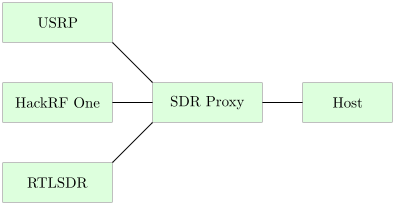
\includegraphics[width=0.5\textwidth]{figures/device_host_usb_interface_fw}
  \caption{Support for multiple types of \gls{SDR} devices.}
  \label{fig:device_host_usb_interface_fw}
\end{figure}
\item A better pipeline for incoming samples.

  Samples are currently fetched in chunks that forces the analyzer to
  lose synchronization when all samples in a chunk is completely
  processed. A better pipeline could be based on the approach GNU
  Radio uses, by having a scheduler that keeps track of ingoing and
  outgoing samples. Each module must inform the scheduler if it
  consumes any samples and if that is the case, the supplied pointer
  of the sample buffer is incremented.

\item Support for decoding and decryption of speech frames.

  Only dedicated user traffic is encrypted, and such a feature can be
  added by supporting the verified implementation of A5/1, reverse
  engineered by Smartcard Developer Association~\cite{a51decryption}.

\item Decoding of \gls{SMS} messages, as they are fetched by a mobile
  phone on the current monitored channel.
\item \gls{GSM} specifies frequency hopping as an optional feature and
  it might be a necessity for the procotol analyzer in certain areas
  to remain synchronized.
\item Fully implement all extractable information of \gls{GSM} layer
  three protocols.
\item The analyzer was designed for multiple mobile technologies in
  mind, thus these were intended to be easy to implement in the
  future. This project could be a base for future bachelor projects.
\begin{figure}[H]
  \centering
  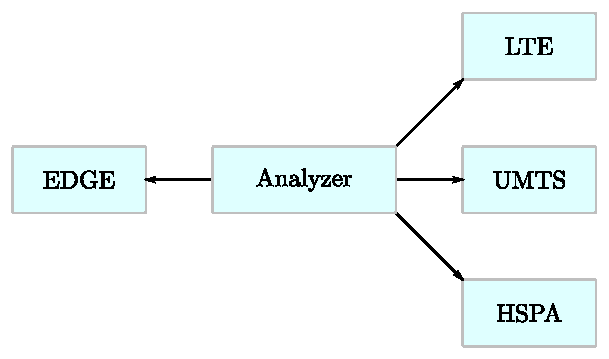
\includegraphics[width=0.5\textwidth]{figures/analyzer_interface_fw}
  \caption{An evolved version of the analyzer with support for
    the upgraded \gls{GSM} technology, EDGE, and the third and fourth
    generation mobile technologies.}
  \label{fig:analyzer_interface_fw}
\end{figure}
\end{itemize}
